
\documentclass [xcolor=x11names,t] {beamer} 


%====================================================
%================== TIKZ  ===========================
%====================================================


\usepackage{tikz,times}
\usepackage{geometry}

\usetikzlibrary{mindmap,backgrounds}
\usepackage{xcolor,colortbl}
%%%%%%%%%%%%%%%%%%%%%%%%%%%%%%%%%%%%%%%%%%%%%%%%%%%%%%%%%%%%%%%%%%
%                                                                %
%                                                                %
%             PACKAGE    UFC - SD                                 %
%                                                                %
%            Auteur : Dorine Tabary                              %
%            Tiré du template Université Paris-Saclay            % 
%                         de Auriane Gabaut                      %
%                                                                %
%%%%%%%%%%%%%%%%%%%%%%%%%%%%%%%%%%%%%%%%%%%%%%%%%%%%%%%%%%%%%%%%%%

%  Basique :

\usepackage[utf8]{inputenc}
\usepackage[T1]{fontenc}
\usepackage[french]{babel} 
\usepackage{hyperref}                           %référence
%\usepackage[margin=1,25cm]{geometry}           %Géométrie

% Mathématiques :
\usepackage{cancel}                             %rayer 
\usepackage{amsthm,amsmath,amsfonts,amssymb,dsfont}    %maths et joli....
\usepackage{stmaryrd}                           %crochet entre autre

% Mise en forme : 

\usepackage[x11names]{xcolor}                   % inclus les couleurs
\usepackage{enumitem}                           % Énumération avec label
\usepackage{multicol}                           % Colonne
\usepackage{graphicx}                           % Pour le bigcdot notamment
\usepackage{tcolorbox}                          % Box
\setlength{\fboxrule}{3pt}
\setlength{\fboxsep}{1em}




% Figure et Image :

\usepackage{wrapfig}                            %pour inclure des figures dans le texte  

%Lettres grecques :
\usepackage{savesym}
\usepackage{amsmath, amssymb}
\savesymbol{iint}
\usepackage{txfonts,, newtxmath}
\restoresymbol{TXF}{iint}
%\usepackage{mathptmx} %uses times fontv

%Beamer
\usepackage{booktabs, comment} 
\usepackage[absolute, overlay]{textpos}
\usepackage{pgfpages}
\usepackage[font=footnotesize]{caption}
\useoutertheme{infolines} 
\usepackage{csquotes}
\usepackage{textpos}
\usepackage{tikz}

%%%%%%%%%%%%%%%%%%%%%%%%%%%%%%%%%%%%%%%%%%%%%%%%%%%%%%%%%%%%%%%%%%
%                                                                %
%                                                                %
%                       Théorème                                 %
%                                                                %
%                                                                %
%%%%%%%%%%%%%%%%%%%%%%%%%%%%%%%%%%%%%%%%%%%%%%%%%%%%%%%%%%%%%%%%%%

\newtheorem*{remark}{Remark}

\theoremstyle{plain}% default
\newtheorem{Th}{Théorème}[section]
\newtheorem{Lem}[Th]{Lemme}
\newtheorem{Prop}[Th]{Proposition}
\newtheorem*{Prop*}{Proposition}
\newtheorem*{Cor}{Corollaire}
\newtheorem*{Obj}{Objection}

\theoremstyle{definition}
\newtheorem{Df}{Définition}[section]
\newtheorem*{Df*}{Définition}
\newtheorem{Dfs}[Df]{Définitions}%[section]
\newtheorem{conj}{conjecture}[section]
\newtheorem{Ex}{Exemple}[section]
\newtheorem*{Ex*}{Exemple}
\newtheorem{Exs}[Ex]{Exemples}%[section]

\theoremstyle{remark}
\newtheorem*{NB}{Remarque}
\newtheorem*{NBs}{Remarques}
\newtheorem*{Gen}{Généralisation}
\newtheorem*{nota}{Notation}
\newtheorem*{Rap}{Rappel}


\renewcommand{\proofname}{\textsc{Preuve}}

\newtheoremstyle{exostyle}{\topsep}{\topsep}{}{}{\bfseries}{.}{ }{\thmname{#1}\thmnumber{ #2}\thmnote{. \normalfont{\textit{#3}} }}

\theoremstyle{exostyle}
\newtheorem{exercice}{Exercice} 

\newtheoremstyle{exostyle}{\topsep}{\topsep}{}{}{\bfseries}{.}{ }{\thmname{#1}\thmnumber{ #2}\thmnote{. \normalfont{\textit{#3}}}}

\theoremstyle{exostyle}
\newtheorem*{preuve}{Preuve} 

\newenvironment{questions}{\begin{enumerate}}{\end{enumerate}}
\newenvironment{sousquestions}{\begin{enumerate}}{\end{enumerate}}

%%%%%%%%%%%%%%%%%%%%%%%%%%%%%%%%%%%%%%%%%%%%%%%%%%%%%%%%%%%%%%%%%%
%                                                                %
%                                                                %
%                       Code                                     %
%                                                                %
%                                                                %
%%%%%%%%%%%%%%%%%%%%%%%%%%%%%%%%%%%%%%%%%%%%%%%%%%%%%%%%%%%%%%%%%%

\usepackage{color}
\usepackage{listings}
\definecolor{mygreen}{rgb}{0,0.6,0}
\definecolor{mygray}{rgb}{0.5,0.5,0.5}
\definecolor{mymauve}{rgb}{0.58,0,0.82}
\definecolor{myorange}{rgb}{0.855,0.576,0.027}
\lstset{
language=Octave,
frame=single,   
morecomment = [l][\itshape\color{blue}]{\%},
keywordstyle=\color{blue},
commentstyle=\color{mygreen},
breakatwhitespace=false,         
breaklines=true,  
numbers=left,
numbersep=5pt,
numberstyle=\tiny\color{mygray}, 
showstringspaces=false,
showtabs=false,                  
tabsize=2,
stringstyle=\color{myorange},
title=\lstname,
literate=
{+}{{{\color{red}+}}}
{-}{{{\color{red}-}}}
{*}{{{\color{red}*}}}
{,}{{{\color{red},}}}
{=}{{{\color{red}=}}}
{(}{{{\color{black}(}}}
{)}{{{\color{red})}}}
{;}{{{\color{red};}}}
{:}{{{\color{red}:}}}
{[}{{{\color{red}[}}}
{]}{{{\color{red}]}}}
{>}{{{\color{red}>}}}
}

%%%%%%%%%%%%%%%%%%%%%%%%%%%%%%%%%%%%%%%%%%%%%%%%%%%%%%%%%%%%%%%%%%
%                                                                %
%                                                                %
%                       Commandes                                %
%                                                                %
%                                                                %
%%%%%%%%%%%%%%%%%%%%%%%%%%%%%%%%%%%%%%%%%%%%%%%%%%%%%%%%%%%%%%%%%%

\newcommand{\N}{\mathbb{N}}
\newcommand{\Z}{\mathbb{Z}}
\newcommand{\R}{\mathbb{R}}
\newcommand{\C}{\mathbb{C}}
\newcommand{\D}{\mathcal D}
\newcommand{\Cl}{\mathcal C}
\newcommand{\Sm}{S^m_{0,1}}
\newcommand{\et}{\text{ ~et~ }}
\newcommand{\ou}{\text{ ~ou~ }}
\newcommand{\espace}{\vspace*{1cm}}
\everymath{\displaystyle}
\renewcommand{\Im}{\text{Im}}
\renewcommand{\Re}{\text{Re}}
\makeatletter
\newcommand*\bigcdot{\mathpalette\bigcdot@{.4}}
\newcommand*\bigcdot@[2]{\mathbin{\vcenter{\hbox{\scalebox{#2}{$\m@th#1\bullet$}}}}}
\makeatother

\newcommand{\framewithtitle}[1]{
\begin{frame}[c]{  }
\Huge{
\begin{center}
    \begin{tcolorbox}[arc=1ex, colback=myuniversity, colframe=myuniversity, left=3pt, right=3pt, top=3pt, bottom=2pt]
    \emph{
    \espace
    \begin{center}
        \textcolor{white}{#1}
    \end{center}
    \espace}
    \end{tcolorbox}
\end{center}}
\end{frame}
}

%%%%%%%%%%%%%%%%%%%%%%%%%%%%%%%%%%%%%%%%%%%%%%%%%%%%%%%%%%%%%%%%%%
%                                                                %
%                                                                %
%                       Beamer                                   %
%                                                                %
%                                                                %
%%%%%%%%%%%%%%%%%%%%%%%%%%%%%%%%%%%%%%%%%%%%%%%%%%%%%%%%%%%%%%%%%%



%% lien vers celui de janvier : https://fr.overleaf.com/8125717386bqbmvyhtchbt

\definecolor{whitetxt}{RGB}{255,255,255}
\definecolor{bluewhite}{RGB}{188,156,196}

\setbeamercolor{title in head/foot}{bg=bluewhite, fg=whitetxt}
\setbeamercolor{author in head/foot}{bg=myuniversity}
\setbeamertemplate{page number in foot}{}

\usetheme{Madrid}
\definecolor{myuniversity}{RGB}{101,35,131}
\usecolortheme[named=myuniversity]{structure}
\usepackage{tikz}


%\addtobeamertemplate{navigation symbols}{}{%
%    \usebeamerfont{footline}%
%    \usebeamercolor[fg]{footline}%
%    \hspace{1em}%
%    \insertframenumber/\inserttotalframenumber
%}

\logo{
\includegraphics[height=1.0cm]{logoF.png}~%
}

\title[Rentrée 2023]{Rentrée 2023 : Bienvenue en première année }
\institute[]{%B.U.T. Sciences des Données \\Université de Franche-Comté
}
\titlegraphic{
\includegraphics[height=1.5cm]{LogoUFC.png}} %mettre celui de votre département 
\author[Dorine Tabary, Cédric Frambourg]{
	B.U.T. - Sciences des données}
\date{11 septembre 2023 }


\begin{document}
\begin{frame}
\maketitle
\end{frame}

%\begin{frame}
%\frametitle{Plan de la Présentation}
%\setcounter{tocdepth}{2}
%\tableofcontents
%\end{frame}


%%%%%%%%%%%%%%%%%%%%%%%%%%%%%%%%%%%%%
%\framewithtitle{Présentation}
\section{Présentation}
\begin{frame}{Présentation de l'équipe}
\begin{block}{Qui sommes-nous ?}


Cédric Frambourg : directeur de département \textcolor{blue}{cedric.frambourg@univ-ubs.fr}    

\begin{itemize}
    \item \textcolor{gray}{supervision des spécialités proposées par le département}
    \item \textcolor{gray}{organisation des programmes et des activités pédagogiques}
   \item  \textcolor{gray}{développement de partenariats avec l'industrie}
\end{itemize}

Dorine Tabary : directrice des études \textcolor{blue}{dorine.tabary@univ-fcomte.fr}

\begin{itemize}
    \item \textcolor{gray}{organisation des cours, des examens et des emplois du temps}
    \item \textcolor{gray}{gestion des questions liées à la réussite scolaire}
    \item \textcolor{gray}{suivi des aménagements pour les étudiants}
\end{itemize}
\end{block}

\begin{alertblock}{En cas de problème :}

Adresse mail : \textcolor{blue}{dorine.tabary@univ-fcomte.fr}
\end{alertblock}


\end{frame}

\begin{frame}{Lieu d'accueil : le Lycée Duhamel}

\begin{block}{Responsables}


Nathalie Kerbeci : proviseure \textcolor{blue}{proviseure@lycee-duhamel.fr}    
\begin{itemize}
    \item \textcolor{gray!50!red}{respect des règles du lycée}
    \item \textcolor{gray}{déplacements : 7h45 à 19h avec un QR-code}

\end{itemize}


Fabrice Favero : directeur délégué aux formations \textcolor{blue}{fabrice.favero@ac-besancon.fr}    


\end{block}

\begin{alertblock}{Repas}

Corinne Chaumette : repas \textcolor{blue}{corinne.chaumette@ac-besancon.fr}    
\begin{itemize}
    \item \textcolor{gray}{gestion des bornes de réservation}
    \item \textcolor{gray}{explication du protocole de réservation}
\end{itemize}
\textbf{Reservation au plus tard la veille pour le lendement.}
\end{alertblock}



\end{frame}


\begin{frame}{Le B.U.T. - Sciences des Données }
    

\begin{minipage}{0.5\textwidth}
\begin{block}{Situation  en France}
15 IUT proposant le BUT-SD
  
\begin{figure}
    \centering
    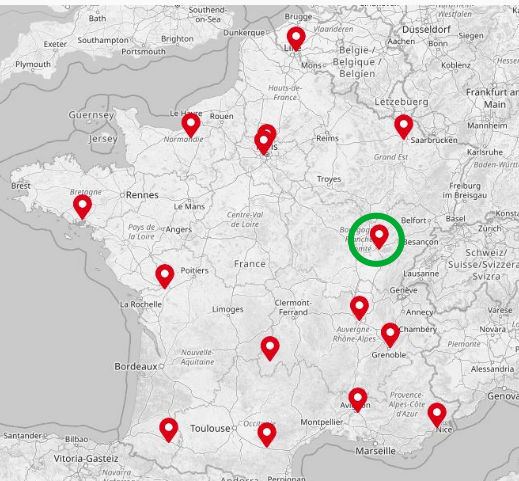
\includegraphics[scale=0.3]{img/dole.png}
\end{figure}
\end{block}
\end{minipage}\hfill
\begin{minipage}{0.45\textwidth}
\begin{block}{La formation}

     \begin{itemize}
        \item 1ère année
        \item effectifs de 15 étudiants
    \end{itemize}


\begin{itemize}
    \item \textbf{savoir}
     \begin{itemize}
        \item informatique
        \item mathématiques
    \end{itemize}
    \item \textbf{savoir être}
     \begin{itemize}
        \item communication
        \item entreprise
    \end{itemize} 
    \item \textbf{savoir faire} 
     \begin{itemize}
        \item alternances
        \item stages
    \end{itemize}   
\end{itemize}
\end{block}

\end{minipage}
\end{frame}

%%%%%%%%%%%%%%%%%%%%%%%%%%%%%%%%%%%%%
\begin{frame}{Les formations de l'IUT à Dole} %[allowframebreaks] si trop de références

  \begin{center}
    \resizebox{1\textheight}{!}{\begin{tikzpicture}[mindmap,
  level 1 concept/.append style={level distance=130,sibling angle=100},
  extra concept/.append style={color=myuniversity!50,text=black}]

  \begin{scope}[mindmap, concept color=myuniversity]

    % Combinatorics and discrete mathematics 
    \node [concept, text=white] at (5.2,-10.8) 
       { } 
      [clockwise from=150]
      child [concept color=myuniversity!50, minimum size=4cm, level distance=150,  text width=3cm,] {node [concept] (ver) {PACKAGING EMBALLAGE CONDITIONNEMENT (PEC)}}
      %child [concept color=blue!50, level distance=125] 
        %{node [concept] (kab) {Kabatyanski, Tsfasman, Rybakov, Zykin}}
      %child [concept color=blue!50] 
        %{node [concept] (kch) {Kucherov, Roytberg}}
      %child [concept color=blue!50] {node [concept] (raf) {Raffinot}}
      child [concept color=myuniversity!50, level distance=130]
        {node [concept] (ksh) {SCIENCE DES DONNEES (SD) }};

  \end{scope}


\node[draw=none,fill=none, white] at (5.1,-11){\Large \textbf{IUT - Dole} };

\node[draw=none,fill=none, black] at (0.5,-13){\Large \textbf{Rattachée à Besançon} };

\node[draw=none,fill=none] at (0,-15.3){
\includegraphics[bb=0 0 0 0, scale =0.6]{LogoUFC.png}};


\end{tikzpicture}
}
  \end{center}
%\begin{tikzpicture}[mindmap,
  level 1 concept/.append style={level distance=130,sibling angle=100},
  extra concept/.append style={color=myuniversity!50,text=black}]

  \begin{scope}[mindmap, concept color=myuniversity]

    % Combinatorics and discrete mathematics 
    \node [concept, text=white] at (5.2,-10.8) 
       { } 
      [clockwise from=150]
      child [concept color=myuniversity!50, minimum size=4cm, level distance=150,  text width=3cm,] {node [concept] (ver) {PACKAGING EMBALLAGE CONDITIONNEMENT (PEC)}}
      %child [concept color=blue!50, level distance=125] 
        %{node [concept] (kab) {Kabatyanski, Tsfasman, Rybakov, Zykin}}
      %child [concept color=blue!50] 
        %{node [concept] (kch) {Kucherov, Roytberg}}
      %child [concept color=blue!50] {node [concept] (raf) {Raffinot}}
      child [concept color=myuniversity!50, level distance=130]
        {node [concept] (ksh) {SCIENCE DES DONNEES (SD) }};

  \end{scope}


\node[draw=none,fill=none, white] at (5.1,-11){\Large \textbf{IUT - Dole} };

\node[draw=none,fill=none, black] at (0.5,-13){\Large \textbf{Rattachée à Besançon} };

\node[draw=none,fill=none] at (0,-15.3){
\includegraphics[bb=0 0 0 0, scale =0.6]{LogoUFC.png}};


\end{tikzpicture}

\end{frame}


\begin{frame}{Le BUT, une formation propice à l'alternance} 

\begin{block}{Intérêt de l'alternance}
\textbf{Statut de salarié et amélioration du CV}
\begin{itemize}
    \item acquisition de compétences pratiques %    Acquisition de compétences pratiques : L'alternance permet aux étudiants d'acquérir une expérience pratique et concrète dans leur domaine d'études. En travaillant directement sur le terrain, les étudiants développent des compétences professionnelles précieuses et se familiarisent avec les défis réels du monde du travail.
    \item  apprentissage concret %: L'expérience pratique en entreprise complète l'apprentissage théorique dispensé en classe. Les étudiants voient comment les concepts théoriques sont appliqués dans la pratique, ce qui renforce leur compréhension et leur permet de mieux retenir les connaissances.
    \item facilitation de l'insertion professionnelle %: Les étudiants en alternance établissent des liens avec des professionnels de leur domaine dès le début de leur carrière. Cela peut ouvrir des opportunités d'emploi à long terme, car les employeurs sont souvent plus enclins à embaucher des diplômés qu'ils connaissent déjà et qui ont fait leurs preuves en entreprise.
    \item rétribution financière %: Dans le cadre de l'alternance, les étudiants reçoivent généralement une rémunération de l'entreprise pour leur travail. Cela peut aider à couvrir les frais de scolarité et d'autres dépenses, réduisant ainsi la charge financière globale de leurs études.
    \item développement de soft skills %: En travaillant avec des collègues et en interagissant avec des clients ou des partenaires commerciaux, les étudiants en alternance développent des compétences interpersonnelles, de communication et d'adaptabilité essentielles pour réussir dans le monde professionnel.
    \item  possibilité de trouver un emploi après l'obtention du diplôme %: Pour de nombreux étudiants en alternance, l'entreprise dans laquelle ils ont travaillé pendant leur formation peut leur offrir un emploi à temps plein après l'obtention de leur diplôme, étant donné qu'ils ont déjà une expérience de travail et sont bien intégrés dans l'entreprise.
    \item alignement avec les besoins du marché du travail %: L'alternance permet aux établissements d'enseignement de s'assurer que leur programme d'études est en phase avec les besoins actuels du marché du travail. Les étudiants développent des compétences directement recherchées par les employeurs, ce qui augmente leurs chances de réussir professionnellement.
\end{itemize}

\end{block}

\begin{block}{L'alternance en Sciences des Données}
    \begin{itemize}
        \item possible dès le B.U.T. 2
        \item fortement recommandée pour le B.U.T. 3
    \end{itemize}
\end{block}

\end{frame}

\begin{frame}{La recherche à l'université}
   
    \begin{block}{L’université = lieu de découverte (recherche) et de partage (enseignement) des connaissances géré par ses pairs}

\begin{minipage}{0.35\textwidth}
        On y compte des tâches 
        \begin{itemize}
            \item de recherche
            \item de vulgarisation
            \item de recherche
            \item  d’enseignement
            \item  et des tâches administratives
        \end{itemize}
\end{minipage}\hfill
\begin{minipage}{0.61\textwidth}
Vos enseignants peuvent :
\begin{itemize}
    \item être enseignants détachés à l’université (concours d’enseignement : professeurs agrégés, certifés)
    \item avoir un rôle de chercheur (concours d’enseignants-chercheurs : maîtres de conférence, professeurs des universités)
    \item et/ou avoir un rôle d’administration
\end{itemize}

\end{minipage}

    \end{block}
\begin{alertblock}{Conclusion}
Les enseignants ne sont pas toujours disponibles pour vous car sollicités sur d’autres missions 
=> 

\textbf{Prise de rendez-vous si vous souhaitez échanger avec un enseignant}
    
\end{alertblock}
    
\end{frame}

\begin{frame}{L'équipe SD 2023/2024}

\begin{minipage}{0.4\textwidth}
\begin{block}{Secrétariat}
    ???
\end{block}
\begin{block}{Statistique}
    Cédric \textbf{Frambourg},
    \begin{itemize}
        \item \textcolor{gray!50!black}{\textit{enseignant}}
    \end{itemize}
\end{block}
\end{minipage}\hfill
\begin{minipage}{0.55\textwidth}
\begin{block}{Informatique}
    Dorine \textbf{Tabary},
    \begin{itemize}
        \item \textcolor{gray!50!black}{\textit{enseignant-chercheur}}
    \end{itemize}
    Nicolas \textbf{Marilleau}
    \begin{itemize}
        \item \textcolor{gray!50!black}{\textit{enseignant-chercheur}}
    \end{itemize}
    Mohammed \textbf{Azerkane}, 
    \begin{itemize}
        \item \textcolor{gray!50!black}{\textit{enseignant pro}}
    \end{itemize}
\end{block}
\begin{block}{Enseignements généraux}
Sandrine \textbf{Thomas}, 
    \begin{itemize}
        \item \textcolor{gray!50!black}{\textit{enseignant pro - communication}}
    \end{itemize}
\end{block}
\end{minipage}
    
\end{frame}

\begin{frame}{Réseaux de la formation  Sciences des Données} %[allowframebreaks] si trop de références
\begin{block}{Réseaux d'étudiants}
    Discord
    
    ???
\end{block}
\begin{block}{Réseaux universitaires}
   Facebook Université de Franche-Comté :
   
   \small \textcolor{myuniversity}{\url{https://www.facebook.com/universiteFrancheComte}}
\end{block}

\end{frame}



\begin{frame}{Planning de l'année : disponible sur l'ENT} %[allowframebreaks] si trop de références
\scriptsize
\begin{minipage}{0.45\textwidth}
\begin{tabular}{|c|c|c|}\hline
     \textbf{Du}& \textbf{Au}& \textbf{1ère année} \\ \hline
     \cellcolor{myuniversity!30}11 sept&\cellcolor{myuniversity!30} 17 sept&  \cellcolor{myuniversity!30} Rentrée\\ \hline
     18 sept& 24 sept&  \\ \hline
     25 sept& 1 oct &  \\ \hline
     \cellcolor{red!30} 2 oct& \cellcolor{red!30} 8 oct& \cellcolor{red!30} Evaluation\\ \hline
     9 oct& 15 oct&  \\ \hline
     \cellcolor{red!30} 16 oct& \cellcolor{red!30} 22 oct&  \cellcolor{red!30} Evaluation\\ \hline
     \cellcolor{green!30}23 oct& \cellcolor{green!30}29 oct& \cellcolor{green!30} Vacances \\ \hline
     \cellcolor{green!30}30 oct&\cellcolor{green!30} 5 nov& \cellcolor{green!30} Vacances\\ \hline
     \cellcolor{red!30} 6 nov& \cellcolor{red!30} 12 nov& \cellcolor{red!30} Evaluation\\ \hline
    \cellcolor{red!30} 13 nov&\cellcolor{red!30} 19 nov& \cellcolor{red!30} Evaluation\\ \hline
     20 nov& 26 nov&  \\ \hline
     27 nov& 3 dec&  \\ \hline
     4 dec& 10 dec&  \\ \hline
     \cellcolor{red!30}11 dec& \cellcolor{red!30}17 dec& \cellcolor{red!30} Evaluation \\ \hline
     \cellcolor{red!30}18 dec&\cellcolor{red!30} 24 dec& \cellcolor{red!30} Evaluation \\ \hline
     \cellcolor{green!30}25 dec& \cellcolor{green!30}31 dec&\cellcolor{green!30} Vacances \\ \hline
     \cellcolor{green!30}1 jan&\cellcolor{green!30} 7 jan &\cellcolor{green!30} Vacances \\ \hline\hline
     \cellcolor{red!30}8 jan& \cellcolor{red!30}14 jan &  \cellcolor{red!30}Evaluation\\ \hline
     \cellcolor{red!30}15 jan&\cellcolor{red!30} 21 jan& \cellcolor{red!30} Evaluation\\ \hline
\end{tabular}
\end{minipage}\hfill
\begin{minipage}{0.45\textwidth}
\begin{tabular}{|c|c|c|}\hline
     22 jan& 28 jan&  \\ \hline
     29 jan& 4 fev &  \\ \hline
     5 fev & 11 fev& \\ \hline
     \cellcolor{red!30}12 fev & \cellcolor{red!30}18 fev&\cellcolor{red!30} Evaluation \\ \hline
     \cellcolor{green!30}19 fev & \cellcolor{green!30}25 fev& \cellcolor{green!30}Vacances \\ \hline
     \cellcolor{green!30}26 fev & \cellcolor{green!30}3 mars&  \cellcolor{green!30}Vacances \\ \hline
      \cellcolor{red!30}4 mars&  \cellcolor{red!30}10 mars&\cellcolor{red!30}  Evaluation\\ \hline
     11 mars&  17 mars&  \\ \hline
     18 mars&  24 mars&  \\ \hline
     25 mars&  31 mars&  \\ \hline
    \cellcolor{red!30} 1 avr&\cellcolor{red!30} 7 avr& \cellcolor{red!30} Evaluation\\ \hline
     \cellcolor{green!30}8 avr&\cellcolor{green!30} 14 avr& \cellcolor{green!30} Vacances\\ \hline
     \cellcolor{green!30}15 avr& \cellcolor{green!30}21 avr&\cellcolor{green!30} Vacances \\ \hline
     22 avr& 28 avr&  \\ \hline
     29 avr& 5 mai&  \\ \hline
     6 mai& 12 mai&  \\ \hline
     \cellcolor{red!30}13 mai&\cellcolor{red!30} 19 mai& \cellcolor{red!30} Evaluation\\ \hline
     20 mai& 26 mai&  \\ \hline
     \cellcolor{red!30}27 mai& \cellcolor{red!30}2 juin&  \cellcolor{red!30}Evaluation\\ \hline
     \cellcolor{red!30}3 juin& \cellcolor{red!30}9 juin& \cellcolor{red!30}Evaluation\\ \hline
     \cellcolor{red!30}10 juin& \cellcolor{red!30}16 juin&\cellcolor{red!30} Evaluation\\ \hline
\end{tabular}
\end{minipage}
\end{frame}



\begin{frame}{Organisation du travail à l’IUT}

\begin{block}{Organisation}
    Cours du lundi au vendredi de 8h à 19h selon l’emploi du temps
    
Fin des cours le vendredi à 17h15 max

Finalisation des emplois du temps possible jusqu’à l’avant-veille    
\end{block}

\begin{block}{ Approche par compétences}
    Le BUT STID est découpé en 2 \textbf{parcours}

Le BUT est un diplôme structuré en \textbf{compétence}

Chaque parcours comporte 4 \textbf{compétences} (4 unités d’enseignements)

Chaque compétence est déclinée en 2 ou 3 \textbf{niveaux de développement} (1 niveau par année)

Chaque compétence contient des \textbf{apprentissages critiques} (à acquérir pour attester de son niveau de compétence)
\end{block}

\end{frame}


\begin{frame}{Approche par compétence}
	\begin{block}{Description}
	Les compétences s’acquièrent en attestant de sa capacité à la mettre en œuvre en répondant à des \textbf{situations professionnelles}.
	
	Pour attester de cette capacité, l’étudiant rencontre des \textbf{Situations d’Apprentissage et 
	d’Évaluation} aussi appelées SAÉ.
	
	Une SAÉ prendra la forme d’un projet, d’un TP, d’une série de TP...
	Pour mener à bien la réalisation de ses compétences, l’étudiant accède à des \textbf{ressources} (les enseignements).
	
	
	Dans le cadre de la formation, l’étudiant construit un portfolio, où il apportera les preuves de l’acquisition de tous les \textbf{apprentissages critiques}.
	\end{block}
	
\end{frame}

\begin{frame}{Validation du BUT}
	\begin{block}{Obtention du diplôme}
	La validation du BUT nécessite la validation des 3 années qui le composent

	La validation d’une année nécessite la validation des compétences qui la composent

	Les enseignements sont organisés en compétences sur six semestres, chaque compétence est déclinée chaque année en niveau 

	La validation d’un niveau de compétence s’obtient
	\begin{itemize}
		\item lorsque la moyenne des notes des deux semestre est >10
		\item lorsqu’on valide le niveau supérieur (année suivante) de la compétence
	\end{itemize} 
		
	\end{block}

\end{frame}

\begin{frame}{IUT et règlement}
	\scriptsize
	\begin{itemize}
	\item Règlement intérieur
	\item Prévention et lutte contre le bizutage
	\item	Sécurité informatique : droits \& devoirs
	\end{itemize}	
	
	\begin{block}{Prévention et lutte contre le bizutage}

		Extrait de la lettre de la Ministre, G. Fioraso, en date du 30/07/2013
" ... Parce qu’il reste, dans l’esprit de beaucoup, une certaine ambiguïté quant à la portée exacte de la réglementation pénale, je tiens à rappeler quelques éléments de droit :
\begin{itemize}
	\item Tous les actes de bizutage sont interdits ;
	\item Le libre consentement des participants ne suffit pas à absoudre les responsables ;
	\item Les personnes morales peuvent être déclarées responsables pénalement des infractions et la responsabilité du chef d’établissement peut être engagée, que l’événement se déroule ou non au sein de l’établissement :
	\item 	Les auteurs des faits ne sont pas les seuls à pouvoir être poursuivis : toute personne qui, par son comportement, encourage ou facilite le bizutage, participe à son organisation ou s’abstient d’intervenir pour l’empêcher est susceptible d’être poursuivie.
	
\end{itemize}


Les temps d’accueil ou d’intégration, qu’ils se déroulent sur une ou plusieurs journées, se doivent d’être exclusivement des temps d’information, d’échange et de convivialité pour être utiles et bénéfiques.		
	\end{block}
	
\end{frame}
\scriptsize
\begin{frame}{Sécurité informatique : droits \& devoirs}
	\begin{itemize}
		\item \textbf{But} : assurer à chacun l’utilisation optimale des ressources compte-tenu des contraintes globales imposées par leur partage.
		\item \textbf{Portée} : année universitaire.
		\item \textbf{Objet} : 
		\begin{itemize}
			\item utilisation des ressources informatiques de l’UFR ;
			\item utilisation des ressources accessibles via le réseau RENATER (Réseau National de Télécommunications pour la Technologie, l’Enseignement et la Recherche) ;
			\item dispositions législatives et sanctions ;
			\item principes déontologiques.
		\end{itemize}
		\item \textbf{Engagements }:
		\begin{itemize}
			\item ne pas masquer sa véritable identité ;
			\item ne pas obtenir le mot de passe d’un autre utilisateur ;
			\item ne pas altérer les données ou accéder à des informations appartenant à un autre utilisateur ;
			\item ne pas porter atteinte à l’intégrité d’un autre utilisateur, par l’intermédiaire de messages, images ou textes provocants ;
			\item ne pas interrompre le fonctionnement normal du réseau ou de l’un de ses composants ;
			\item ne pas modifier les paramètres des systèmes connectés au réseau ;
			\item ne pas télécharger d’œuvres protégées ;
			\item ne pas envoyer en masse des courriels non-sollicités (SPAM/Pourriels) ;
			\item ne pas consulter de sites contraires à l’éthique de l’université ;
			\item ne pas utiliser de logiciel permettant de tels agissements.
			
		\end{itemize} 
		

	\end{itemize}
\end{frame}

\begin{frame}{Nul n'est censé ignorer la loi}
		 \textbf{Code pénal article 323-1} :
		 
		Le fait d'accéder ou de se maintenir, frauduleusement, dans tout ou partie d'un système de traitement automatisé de données est puni de \textbf{deux ans d'emprisonnement et de 30000 euros d'amende}. 
		
		Lorsqu'il en est résulté soit la suppression ou la modification de données contenues dans le système, soit une altération du fonctionnement de ce système, la peine est de \textbf{trois ans d'emprisonnement et de 45000 euros d'amende}.
		
		Lorsque les infractions prévues aux deux premiers alinéas ont été commises à l'encontre d'un système de traitement automatisé de données à caractère personnel mis en œuvre par l'Etat, la peine est portée à \textbf{cinq ans d'emprisonnement et à 75 000 € d'amende}.

	\textbf{Code pénal article 323-2} :

		Le fait d'entraver ou de fausser le fonctionnement d'un système de traitement automatisé de données est puni de \textbf{cinq ans d'emprisonnement et de 75000 euros d'amende}. Lorsque cette infraction a été commise à l'encontre d'un système de traitement automatisé de données à caractère personnel mis en œuvre par l'Etat, la peine est portée à sept ans d'emprisonnement et à \textbf{100 000 € d'amende}.
	
	\textbf{Code pénal article 323-3} :
	
		Le fait d'introduire frauduleusement des données dans un système de traitement automatisé ou de supprimer ou de modifier frauduleusement les données qu'il contient est puni de \textbf{cinq ans d'emprisonnement et de 75000 euros d'amende}. Lorsque cette infraction a été commise à l'encontre d'un système de traitement automatisé de données à caractère personnel mis en œuvre par l'Etat, la peine est portée à \textbf{sept ans d'emprisonnement et à 100 000 € d'amende}.
	

\end{frame}

\begin{frame}{Nul n'est censé ignorer la loi}
		\textbf{Code pénal article  323-4} :
		La participation à un groupement formé ou à une entente établie en vue de la préparation, caractérisée par un ou plusieurs faits matériels, d'une ou de plusieurs des infractions prévues par les articles 323-1 à 323-3-1 est punie des peines prévues pour l'infraction elle-même ou pour l'infraction la plus sévèrement réprimée.
		
		\textbf{Code pénal article 323-5} :
		 Les personnes physiques coupables des délits prévus au présent chapitre encourent également les peines complémentaires suivantes :
		\begin{itemize}
			\item L'interdiction, pour une durée de cinq ans au plus, des droits civiques, civils et de famille, suivant les modalités de l'article 131-26 ;
			\item L'interdiction, pour une durée de cinq ans au plus, d'exercer une fonction publique ou d'exercer l'activité professionnelle ou sociale dans l'exercice de laquelle ou à l'occasion de laquelle l'infraction a été commise ;
			\item La confiscation de la chose qui a servi ou était destinée à commettre l'infraction ou de la chose qui en est le produit, à l'exception des objets susceptibles de restitution ; 
			\item La fermeture, pour une durée de cinq ans au plus, des établissements ou de l'un ou de plusieurs des établissements de l'entreprise ayant servi à commettre les faits incriminés ;
			\item L'exclusion, pour une durée de cinq ans au plus, des marchés publics ;
			\item L'interdiction, pour une durée de cinq ans au plus, d'émettre des chèques autres que ceux qui permettent le retrait de fonds par le tireur auprès du tiré ou ceux qui sont certifiés ;
			\item L'affichage ou la diffusion de la décision prononcée dans les conditions prévues par l'article 131-35.
		\end{itemize}
		
	
\end{frame}

\begin{frame}{Nul n'est censé ignorer la loi}

\begin{center}
	\LARGE
	\textcolor{red}{Adoptez une attitude responsable et raisonnable}
	
\end{center}	
	
\end{frame}
\normalsize

\begin{frame}{Médecine préventive / services sociaux}
	\begin{block}{Rendez vous possibles avec :}
	\begin{itemize}
		\item Le Service d’Accompagnement des Étudiants en Situation de Handicap (SAESH) : aménagement d’étude
		\item Une assistante de service social étudiant : accueil et écoute des étudiants en difficulté, quelle qu'en soit la nature : familiale, financière ou administrative
	\end{itemize}		 
		
	\end{block}
	
	
	\begin{center}
		\LARGE
		\textcolor{myuniversity}{Merci de votre attention : des questions ?}
		
	\end{center}	
	
	
\end{frame}

%%%%%%%%%%%%%%%%%%%%%%%%%%%%%%%%%%%%%
%\begin{frame}{Références} %[allowframebreaks] si trop de références
%\nocite*
%\tiny
%\bibliographystyle{apalike}
%\bibliography{ref}
%\end{frame}


\end{document}